\documentclass[11pt,a4paper]{article}
\usepackage[utf8x]{inputenc}
\usepackage{graphicx}
\usepackage[english]{babel}
\usepackage{color}
\usepackage{fontspec}
\usepackage{float}
\usepackage{caption}
\usepackage{subcaption}
\usepackage{mathtools}
\usepackage{algorithm2e}

\usepackage[colorlinks=true]{hyperref} % the option is there to remove the square around links which is what I don't like.

\usepackage{perpage} 
\MakePerPage{footnote} % Reset the footnote counter perpage. may require to run latex twice.

\usepackage[margin=2cm]{geometry} % This is here to fit more text into the page.

\setcounter{secnumdepth}{1}  % This removes the numbering from the subsections.
                        % If you want the numbering of the subsection level just remove this line

\title{\textsc{Assignment Title}}
\author{    Yasser Souri\thanks{Anyone to thank?} \ (\textit{stdnum}) \\
        Department of Computer Engineering\\
        Sharif University of Technology\\
        \texttt{ysouri@ce.sharif.edu}}
\date{}

\setlength{\parindent}{0pt} % No indentation for paragraphs. Because that is just old.
\setlength{\parskip}{\baselineskip} % Instead use vertical paragraph spacing.

\fontencoding{T1} % the better font encoding.

%\setmainfont{Helvetical} % Setting the main font here. But I like the default font alot so this is commented out.

\begin{document}
\maketitle

\begin{abstract}
Do we really need an abstract?\footnote{We usually don't have abstracts in assignments but for the sake of it I've put it here.}
Since we have created one, let's do a link to \href{https://github.com/yassersouri}{my github account}.
\end{abstract}


\section{First Section}

Code for this subsection could be found in \texttt{q\_1.m} file in the \texttt{src} folder.

\subsection{A}
This is the answer to question a. √ % just a unicode character to see if everything works fine.
\TeX{} is a computer program for typesetting documents, created by Donald Knuth. It takes a suitably prepared computer file and converts it to a form which may be printed on many kinds of printers, including dot-matrix printers, laser printers and high-resolution typesetting machines. \LaTeX{} is a set of macros for \TeX{} that aim.

This is the next paragraph.
\subsection{B}
Here we show how to embed one diagram as a figure. Take a look at figure \ref{fig:awesome_result}.

\begin{figure}[!h] % the part with "!h" is to place it inside this section. As this is the main way we want to have figures in assignment reports
    \centering
    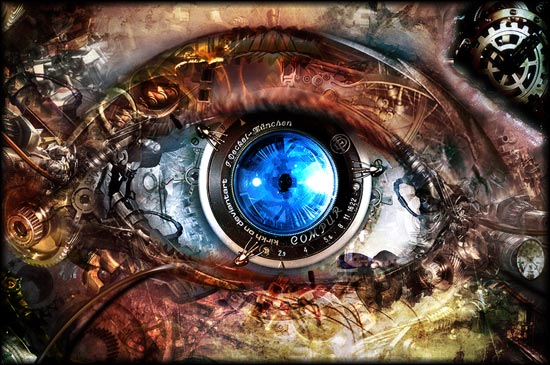
\includegraphics[width=0.3\textwidth]{img.jpg}
    \caption{Awesome Result}
    \label{fig:awesome_result}
\end{figure}


\subsection{C}
Here we show how to embed subfigures as it might be usefull in assignment reports. Take a look at result on figure \ref{fig:multi}.

\begin{figure}[!h] % the part with "!h" is to place it inside this section. As this is the main way we want to have figures in assignment reports
    \centering
    \begin{subfigure}[h]{0.3\textwidth}
        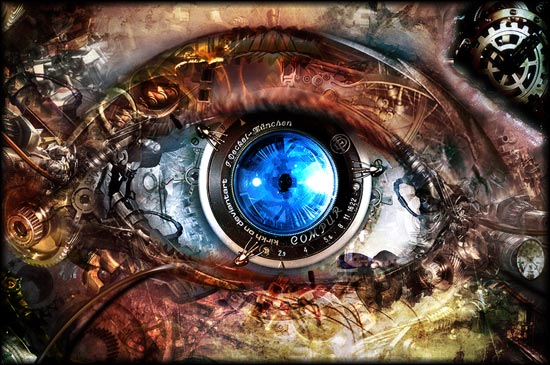
\includegraphics[width=\textwidth]{img}
        \caption{The first}
    \end{subfigure}
    \begin{subfigure}[h]{0.3\textwidth}
        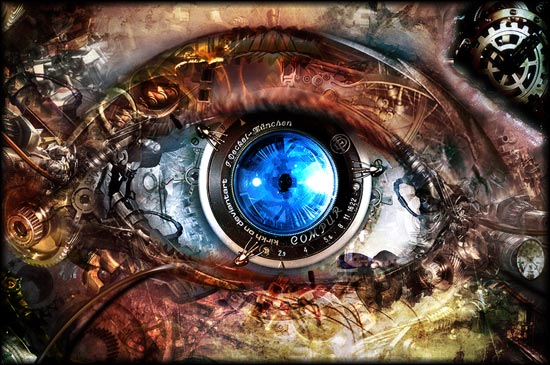
\includegraphics[width=\textwidth]{img}
        \caption{The second}
    \end{subfigure}
    \begin{subfigure}[h]{0.3\textwidth}
        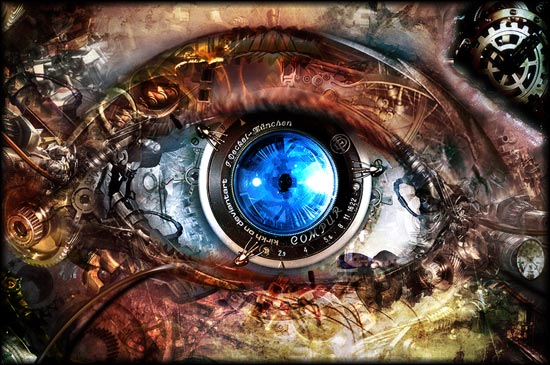
\includegraphics[width=\textwidth]{img}
        \caption{The third}
    \end{subfigure}

    \caption{All of the diagrams}
    \label{fig:multi}
\end{figure}


\subsection{D}
What if we solve the equation \ref{eq}.

\begin{equation}
\label{eq}
x_1 = \frac{5 + \sqrt{25 - 4 \times 6}}{2} = 3
\end{equation}

Also we know that
$
\frac{n!}{k!(n-k)!} = \binom{n}{k}
$ which will help us alot.

\section{Second Section}

Code for this subsection could be found in \texttt{q\_2.m} file in the \texttt{src} folder.

\subsection{A}
We try to solve the problem with Agorithm \ref{alg:first}.

\begin{algorithm}[H]
    \SetAlgoLined
    \KwData{this text}
    \KwResult{how to write algorithm with \LaTeX2e }
    initialization\;
    \While{not at end of this document}{
        read current\;
        \eIf{understand}{
            go to next section\;
            current section becomes this one\;
        }{
        go back to the beginning of current section\;
        }
    }
    \caption{How to write algorithms}
    \label{alg:first}
\end{algorithm}

\subsection{B}
Let's look at the results in Figure \ref{tab:first}
\begin{figure}[!h]
\centering
    \begin{tabular}{ | l | l | l | p{5cm} |}
        \hline
            Day & Min Temp & Max Temp & Summary \\ \hline
            Monday & 11C & 22C & A clear day with lots of sunshine.  
            However, the strong breeze will bring down the temperatures. \\ \hline
            Tuesday & 9C & 19C & Cloudy with rain, across many northern regions. Clear spells
            across most of Scotland and Northern Ireland,
            but rain reaching the far northwest. \\ \hline
            Wednesday & 10C & 21C & Rain will still linger for the morning.
            Conditions will improve by early afternoon and continue
            throughout the evening. \\
        \hline
    \end{tabular}
\caption{The table}
\label{tab:first}
\end{figure}

\end{document}